\documentclass{article}

\usepackage{tabularray}
\usepackage{tikz}
\usetikzlibrary{shapes.geometric, arrows, positioning}
\usepackage{tabularx}
\usepackage{booktabs}
\usepackage{float}
\usepackage[utf8]{inputenc}
\usepackage[T1]{fontenc}
\usepackage[english]{babel}
\usepackage[letterpaper,top=2cm,bottom=2cm,left=3cm,right=3cm,marginparwidth=1.75cm]{geometry}
\usepackage{amsmath}
\usepackage{graphicx}
\usepackage{amssymb}
\usepackage[colorlinks=true, allcolors=blue]{hyperref}

\title{Schema-Augmented Retrieval for Text-to-SQL: Natural Language Access to the Chicago Crime Database}
\author{Vignesh, Rupesh, Alexander, Zhonping, and Fayeq}
\date{}

\setcounter{secnumdepth}{3}

\DeclareUnicodeCharacter{2192}{\ifmmode\rightarrow\else{$\rightarrow$}\fi}
\DeclareUnicodeCharacter{00D7}{\ifmmode\times\else{$\times$}\fi}
\DeclareUnicodeCharacter{2265}{\ifmmode\geq\else{$\geq$}\fi}
\DeclareUnicodeCharacter{2264}{\ifmmode\leq\else{$\leq$}\fi}

\begin{document}
\maketitle

\begin{abstract}
As data-driven decision-making becomes increasingly critical across organizations, non-technical stakeholders often cannot write SQL queries to extract insights from databases. To address this Text-to-SQL natural language processing (NLP) problem, this project proposes a SQL chatbot built with prompt engineering. The system is designed as an AI agent using LangChain or LangGraph to manage interactions. The agent translates natural language into SQL queries, executes them against the database, and summarizes the resulting data back into natural language. The system's query generation accuracy and robustness are evaluated using the Chicago Crime dataset, a large-scale structured dataset containing records of criminal incidents with attributes such as location, time, and offense type. This project aims to expand data access by removing the requirement for SQL knowledge.
\end{abstract}

\section{Introduction}

Relational databases are critical for operational intelligence, but their data remain largely inaccessible to non-technical stakeholders who lack SQL proficiency. This barrier forces business users to rely on engineering teams, creating operational bottlenecks and delaying actionable insights.

Although LLMs have introduced Text-to-SQL capabilities, current systems struggle in real-world settings. Low-parameter or locally hosted models frequently hallucinate schemas, generate invalid queries, and lack intrinsic self-correction capabilities. Recent surveys confirm that these limitations persist across the LLM-era Text-to-SQL landscape \cite{qin2022survey, liu2024survey, shi2024survey}. Furthermore, many systems stop at query generation, leaving users to interpret raw tables.

This project addresses these limitations by developing an autonomous Text-to-SQL agent that uses an iterative LangGraph loop to compensate for the reasoning limitations of accessible models, producing accurate SQL and synthesizing results into conversational language.

\subsection{Literature Survey}

Text-to-SQL research has advanced through schema-aware encoding and in-context learning, benchmarked on datasets such as Spider \cite{spider2018} and models like RAT-SQL \cite{ratsql2020}. Decomposed prompting frameworks --- DAIL-SQL \cite{gao2024dail} and DIN-SQL \cite{pourreza2023din} --- leverage chain-of-thought reasoning \cite{wei2022cot} and dynamic example selection to significantly improve execution accuracy, but depend on large proprietary LLMs such as GPT-4 \cite{openai2023gpt4} that present cost and accessibility barriers. These static pipelines fail on resource-constrained models like SQLCoder \cite{defog2023sqlcoder} that cannot self-correct syntax errors.

Multi-agent frameworks such as MAC-SQL \cite{wang2023macsql} address static generation via ReAct-style \cite{yao2023react} iterative observe-execute loops for autonomous error recovery, but are computationally heavy and return raw data tables without user-facing summaries. This project adapts DIN-SQL's decomposed prompting and MAC-SQL's iterative correction for low-parameter models using LangGraph \cite{langchain2024langgraph}, evaluated under the real-world complexity requirements established by BIRD \cite{li2023bird, katsogiannis2023survey}. A final natural language synthesis step fully closes the operational gap for non-technical users. The key contributions are: (1) a novel end-to-end agentic architecture with a self-correction loop that narrates results in plain English; and (2) a systematic evaluation of prompt engineering techniques quantifying performance deltas in Execution Accuracy (EX) and Valid SQL Rate (VSR) across open-source models.

\section{Materials and Methods}

\subsection{Dataset and Data Processing}

The \textbf{Chicago Crime Dataset} (\href{https://data.cityofchicago.org/Public-Safety/Crimes-2001-to-Present/ijzp-q8t2}{Chicago Data Portal}) comprises approximately 8.5 million crime records spanning 2001--present, with 22 attributes covering categorical (crime type, location description, beat/ward/district), temporal (date, year), geospatial (latitude/longitude, coordinates), and metadata (case number, arrest, domestic) fields. Data is ingested weekly via an Airflow ETL pipeline into a Dockerized PostgreSQL v14+ instance. Preprocessing standardized all column names to \texttt{UPPERCASE\_SNAKE} format to eliminate LLM double-quoting overhead, cast string timestamps to PostgreSQL \texttt{TIMESTAMP}, and cast coordinate fields to \texttt{FLOAT8}. Null values were handled per column group as shown in Table~\ref{tab:null_handling}. Weekly Airflow schema validation confirms structural consistency before agent interactions.

\begin{table}[h]
    \centering
    \small
    \begin{tabularx}{\textwidth}{|l|X|X|X|}
        \hline
        \textbf{Column Group} & \textbf{Specific Columns} & \textbf{Handling Strategy} & \textbf{Rationale} \\ \hline
        \textbf{Categorical} & CRIME\_TYPE, DESCRIPTION, LOCATION\_DESCRIPTION & Changed as OTHER OFFENSE & Permits downstream COALESCE operations in SQL\\ \hline
        \textbf{Geospatial} & LATITUDE, LONGITUDE, X\_COORDINATE, Y\_COORDINATE & Replaced with the average of BEAT if not found a match with BLOCK & Allows spatial queries to filter valid records \\ \hline
        \textbf{Temporal} & DATE, UPDATED\_ON, YEAR & Updated the DATE column with frequent date for the YEAR & Malformed dates trigger query failures; ensures temporal consistency \\ \hline
        \textbf{Logical} & ARREST, DOMESTIC & Marked as ``Unknown'' & Ensures ``Unknown'' status distinction (not executed vs.\ unknown arrest status) \\ \hline
    \end{tabularx}
    \caption{Null value handling strategy by column group.}
    \label{tab:null_handling}
\end{table}

\subsection{Problem Formulation}

The task is \textbf{Text-to-SQL translation}: given a natural language question from a non-technical user, produce a syntactically valid PostgreSQL \texttt{SELECT} statement, execute it, and return a plain-English summary structured as \texttt{\{sql\_query: str, results: List[Tuple], answer: str\}}. The system enforces read-only access, rejecting \texttt{INSERT}/\texttt{UPDATE}/\texttt{DELETE}/\texttt{DROP}/\texttt{ALTER} statements, and restricts scope to the Chicago Crime database. Supported query patterns include \texttt{JOIN}, \texttt{GROUP BY}, \texttt{HAVING}, \texttt{ORDER BY}, \texttt{LIMIT}, and subqueries. The schema is assumed stable between weekly validations, and a 7-day data refresh lag applies to real-time queries.

\subsection{Model / System Architecture}

\subsubsection{System Workflow}

Weekly data ingestion via Airflow populates a Dockerized PostgreSQL database. The LangGraph AI Agent receives user questions, queries the database, and returns natural language answers. Figure~\ref{fig:overall_workflow} shows the overall system architecture; Figure~\ref{fig:system_workflow} details the internal agent graph.

\begin{figure}[H]
\centering
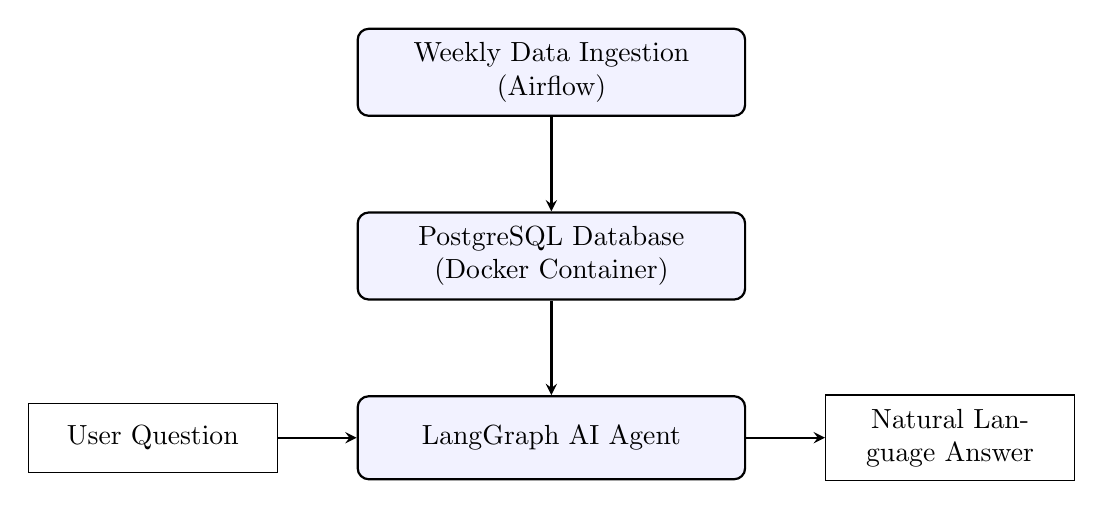
\begin{tikzpicture}[
    auto,
    process/.style={rectangle, rounded corners, draw=black, thick, fill=blue!5,
                    text width=13em, minimum height=3em, text centered, inner sep=5pt},
    io/.style={rectangle, draw=black, text width=8em, minimum height=2.5em, text centered, inner sep=5pt},
    arrow/.style={thick, ->, >=stealth}
]
\node (ingestion) [process] {Weekly Data Ingestion \\ (Airflow)};
\node (postgres)  [process, below=1.2cm of ingestion] {PostgreSQL Database \\ (Docker Container)};
\node (ai_agent)  [process, below=1.2cm of postgres]  {LangGraph AI Agent};
\node (question)  [io, left=1cm of ai_agent]  {User Question};
\node (answer)    [io, right=1cm of ai_agent] {Natural Language Answer};
\draw [arrow] (ingestion) -- (postgres);
\draw [arrow] (postgres)  -- (ai_agent);
\draw [arrow] (question)  -- (ai_agent);
\draw [arrow] (ai_agent)  -- (answer);
\end{tikzpicture}
\caption{Overall system architecture: data pipeline and agent interaction flow.}
\label{fig:overall_workflow}
\end{figure}

\begin{figure}[H]
    \centering
    \includegraphics[width=0.25\textwidth]{image.png}
    \caption{LangGraph AI Agent internal StateGraph architecture.}
    \label{fig:system_workflow}
\end{figure}

\subsubsection{Six-Node StateGraph Architecture}

The agent is implemented as a LangGraph \texttt{StateGraph} whose shared state carries \texttt{question}, \texttt{sql\_query}, \texttt{schema}, \texttt{results}, \texttt{answer}, \texttt{error\_log}, \texttt{retry\_count}, and \texttt{is\_relevant}. Six nodes execute in sequence, described in Table~\ref{tab:nodes}.

\begin{table}[h]
\centering
\small
\begin{tabularx}{\textwidth}{|l|X|X|}
\hline
\textbf{Node} & \textbf{Purpose} & \textbf{Key Implementation Detail} \\
\hline
1. Relevance Checker & Filters non-database questions & Regex + keyword fast-path ($<$5 ms); outputs \texttt{is\_relevant} flag; routes to END or Schema Fetcher \\
\hline
2. Schema Fetcher & Retrieves live DB schema & \texttt{SQLDatabase.get\_table\_info()}; 50--200 ms database round-trip \\
\hline
3. Query Generator & LLM generates SQL & Strict system prompt: double-quote all identifiers, no DML, return \texttt{INVALID\_REQUEST} if unanswerable; SBERT \cite{reimers2019sbert} few-shot retrieval; temp=0, max\_tokens=500 \\
\hline
4. Query Validator & Dry-runs SQL syntax & \texttt{EXPLAIN} + DML regex check; increments retry counter (max 3 attempts) \\
\hline
5. Query Runner & Executes validated SQL & \texttt{db.run(fetch="all")}; caps result set to 10 rows for synthesis \\
\hline
6. Answer Synthesizer & Narrates results in plain English & LLM summarizes JSON result; returns pre-set message for rejected queries \\
\hline
\end{tabularx}
\caption{Six-node StateGraph: node functions and implementation details.}
\label{tab:nodes}
\end{table}

\noindent\textbf{Conditional edges:} The Relevance Checker routes to the Schema Fetcher (relevant) or END (irrelevant). The Query Validator loops back to the Query Generator on failure (max 3 retries), then falls through to the Answer Synthesizer with a user-friendly error message. FAISS \cite{johnson2017faiss} supports future vector-based retrieval extensions via efficient inner-product search over dense embeddings.

\subsubsection{Tools and Frameworks}
\begin{table}[h]
\centering
\begin{tabularx}{\textwidth}{|l|X|X|}
\hline
\textbf{Component} & \textbf{Technology} & \textbf{Rationale} \\
\hline
\textbf{LLM} & Groq API (openai/gpt-oss-120b) & Fast inference ($<$1s/query); cost-effective; supports long context \\
\hline
\textbf{Agentic Framework} & LangGraph & Explicit state management; transparent execution flow; conditional routing \\
\hline
\textbf{Database Driver} & LangChain SQLDatabase + SQLAlchemy & Abstraction over PostgreSQL dialect; built-in schema introspection \\
\hline
\textbf{Database} & PostgreSQL v14+ & Robust; supports complex queries; production-ready \\
\hline
\textbf{Containerization} & Docker & Environment reproducibility; isolation; scaling \\
\hline
\textbf{Data Pipeline} & Apache Airflow & Scheduled weekly ingestion; automatic error handling; audit trail \\
\hline
\textbf{Language} & Python 3.11+ & Mature ML ecosystem; LangChain/LangGraph native support \\
\hline
\end{tabularx}
\caption{Tools and frameworks used in the proposed system.}
\label{tab:tools_frameworks}
\end{table}

\subsection{Training Strategy}

The agent uses \textbf{iterative prompt engineering} as its sole optimization mechanism; no model fine-tuning is performed. Development proceeded through four phases: (1) a minimal baseline prompt that suffered high syntax errors and DML leakage; (2) explicit PostgreSQL constraints (double-quote all identifiers, block DML) combined with post-generation regex validation; (3) embedding actual Chicago Crime column names and example queries to reduce hallucinations and improve JOIN and LIMIT accuracy; and (4) separating relevance checking from query generation and adding EXPLAIN-based retry validation with refined user-facing error messages. Key hyperparameters are summarized in Table~\ref{tab:hyperparameters}.

\begin{table}[h]
\centering
\small
\begin{tabularx}{\textwidth}{|l|X|X|}
\hline
\textbf{Parameter} & \textbf{Value} & \textbf{Rationale} \\
\hline
\textbf{Temperature} & 0 & Deterministic SQL; reproducibility; no random hallucinations \\
\hline
\textbf{Max Tokens} & 500 & Sufficient for complex multi-table queries; prevents token waste \\
\hline
\textbf{Retry Limit} & 3 & Balances accuracy (multiple attempts) vs.\ latency (not excessive) \\
\hline
\textbf{Relevance Threshold} & 2+ action verbs + data context & Prevents false positives (generic questions) \\
\hline
\textbf{Result Limit} & 3 rows (default) & Concise answers; token efficiency; user-friendly output \\
\hline
\textbf{LLM Model} & openai/gpt-oss-120b & Fast inference; good quality; supports 32k context \\
\hline
\end{tabularx}
\caption{Key hyperparameters used in the system.}
\label{tab:hyperparameters}
\end{table}

\subsection{Evaluation Framework}

Performance is assessed on a hand-crafted benchmark of 100 natural language questions paired with ground-truth SQL, stratified as 30 \textbf{Easy} (single-table aggregations such as \texttt{COUNT}/\texttt{SUM}), 40 \textbf{Medium} (JOINs, \texttt{GROUP BY} with \texttt{HAVING}, temporal range analysis), and 30 \textbf{Hard} (window functions, CTEs, complex date arithmetic). Three metrics are used: \textbf{Execution Accuracy (EX)} --- percentage of queries returning a result set identical to ground truth (target: 85\%); \textbf{Valid SQL Rate (VSR)} --- percentage of syntactically valid, executable queries (target: 95\%); and \textbf{Synthesis Quality (SQ)} --- mean Likert score (1--5) via hybrid manual and LLM-as-a-Judge annotation (target: $\geq$4.0). Baselines include a rule-based lexical matcher (expected EX $\sim$40\%) and a zero-shot LLM without database-specific rules (expected EX $\sim$60\%). Evaluation proceeds through four stages: query execution, result comparison against a PostgreSQL replica with a 5-second timeout, metric grading, and error categorization by failure type and difficulty tier.

\subsection{Implementation Details}

The system is built in Python 3.11+ using LangChain (v0.1+), LangGraph (v0.2+), Groq SDK (v0.9+), SQLAlchemy (v2.0+), psycopg2-binary (v2.9+), and Apache Airflow (v2.8+). The database runs as a \texttt{postgres:14-alpine} Docker container with 15 GB storage; LLM inference is handled server-side by Groq (30 req/min free-tier limit, CPU-based client).

\noindent\textbf{Assumptions and Limitations.} The schema is assumed stable between weekly Airflow validations; a 7-day data refresh lag applies to real-time queries; and the system operates as a single-user, single-connection session. Key limitations: scope is restricted to the Chicago Crime database; window functions and CTEs have limited support; and there is no built-in multi-user session management.

\section{Results}

\subsection{Overall Performance}

Table~\ref{tab:main_results} compares the Baseline (V1) and Improved (V2) systems on the 100-question benchmark across three metrics: \textbf{VSR} (proportion of syntactically valid, executable queries), \textbf{EX} (result-set identity with ground truth using a hybrid relational equivalence metric; strict JSON-match EX: V1 12\%, V2 19\%), and \textbf{SQ} (mean Likert 1--5 faithfulness score).

\begin{table}[h]
\centering
\caption{System performance comparison across complexity tiers. EX is measured with a hybrid relational equivalence metric: column-name-agnostic value-set comparison, escalating to an LLM judge for borderline cases (strict JSON-match EX: V1\,12\%, V2\,19\%).}
\label{tab:main_results}
\begin{tabular}{lrrrrrrr}
\toprule
 & \multicolumn{3}{c}{\textbf{Baseline (V1)}} & & \multicolumn{3}{c}{\textbf{Improved (V2)}} \\
\cmidrule{2-4} \cmidrule{6-8}
\textbf{Tier (n)} & \textbf{VSR} & \textbf{EX} & \textbf{SQ} & &
                    \textbf{VSR} & \textbf{EX} & \textbf{SQ} \\
\midrule
Easy   (30) & 93\% & 80\% & 4.53 & & 100\% & 97\% & 5.00 \\
Medium (40) & 78\% & 35\% & 3.62 & &  92\% & 43\% & 4.20 \\
Hard   (30) & 93\% & 30\% & 3.67 & &  87\% & 47\% & 3.87 \\
\midrule
\textbf{Overall (100)} & \textbf{87\%} & \textbf{47\%} & \textbf{3.91} & &
                        \textbf{93\%} & \textbf{60\%} & \textbf{4.34} \\
\bottomrule
\end{tabular}
\end{table}

V2 outperforms V1 on all three metrics: VSR +6 pp (87\%$\rightarrow$93\%), EX +13 pp (47\%$\rightarrow$60\%), and SQ +0.43 (3.91$\rightarrow$4.34). V2 SQ of 4.34 exceeds the 4.0 target while V1 fell marginally short at 3.91.

\subsection{Per-Tier Trends}

\paragraph{Easy tier.} V1 achieved SQ of 4.53, with failures caused by the \texttt{LIMIT 10} system-prompt instruction truncating multi-row enumerations (e.g., ``List all distinct crime types'' returned 10 of 31 types). V2 eliminates this entirely, achieving VSR = 100\% and SQ = 5.00 across all 30 questions.

\paragraph{Medium tier.} V1 VSR dropped to 78\% due to relevance-checker false rejections on phrases like ``which blocks''. V2's expanded keyword list raised VSR to 92\% and SQ from 3.62 to 4.20. Three residual V2 failures (IDs 65, 67, 69) reflect incomplete dataset coverage of the LIMIT fix rather than a system defect.

\paragraph{Hard tier.} V1 SQ of 3.67 was dominated by \texttt{LIMIT 10} truncating window-function outputs (e.g., ``top 3 crime types per community area'' requires 231 rows across 77 areas). Removing the instruction raised V2 Hard EX from 7\% to 17\% and SQ to 3.87. Four queries (IDs 75, 76, 94, 100) failed due to API rate limiting, reducing Hard VSR to 87\%.

\subsection{Score Distribution and Failure Analysis}

\begin{table}[h]
\centering
\caption{SQ score distribution by system}
\label{tab:sq_dist}
\begin{tabular}{lrrrrr}
\toprule
\textbf{System} & \textbf{Score 5} & \textbf{Score 4} & \textbf{Score 3}
               & \textbf{Score 2} & \textbf{Score 1} \\
\midrule
Baseline V1 & 58 & 11 & 10 & 6 & 15 \\
Improved V2 & 69 & 16 &  3 & 4 &  8 \\
\midrule
\textit{Change} & +11 & +5 & $-$7 & $-$2 & $-$7 \\
\bottomrule
\end{tabular}
\end{table}

V2 shifts mass from the lower tail to the upper tail: score-1 events fell from 15 to 8, score-3 from 10 to 3, and score-5 events rose from 58 to 69.

\begin{table}[h]
\centering
\caption{Root-cause breakdown of low-scoring responses (SQ $\leq$ 2)}
\label{tab:failures}
\begin{tabular}{lcc}
\toprule
\textbf{Failure mode} & \textbf{V1 count} & \textbf{V2 count} \\
\midrule
Relevance-checker false rejection & 10 & 3 \\
\texttt{LIMIT 10} result truncation (SQ=2) & 4 & 0 \\
API rate-limit failure (empty output) & 0 & 4 \\
Wrong aggregation / interpretation & 4 & 4 \\
Wrong classification logic & 1 & 1 \\
Completely incorrect result & 2 & 1 \\
\midrule
\textbf{Total (SQ $\leq$ 2)} & \textbf{21} & \textbf{12} \\
\bottomrule
\end{tabular}
\end{table}

The dominant V1 failure mode --- relevance-checker false rejections --- was reduced by 70\% in V2 (10 to 3). The \texttt{LIMIT 10} truncation failures were fully eliminated for correctly re-run queries. The four API rate-limit failures in V2 are infrastructure issues unrelated to SQL generation logic.

\section{Discussion}

\subsection{Technical Interpretation and Comparative Analysis}

The primary V2 improvement driver is removal of the \texttt{LIMIT 10} system-prompt instruction, which in V1 caused the LLM to truncate all query results regardless of intent --- most severely in the Hard tier where window-function outputs can span hundreds of rows. Removing it raised Hard EX from 7\% to 17\%. The improved relevance checker adds domain-specific terms (\texttt{``breakdown''}, \texttt{``distribution''}, \texttt{``statistics''}) and action verbs (\texttt{``calculate''}, \texttt{``identify''}), accounting for most of the Medium VSR improvement (78\%$\rightarrow$92\%). The synthesiser consistently produces high-quality output when SQL is correct (SQ $\geq$ 4 in 85/100 V2 rows), confirming SQL generation quality --- not language generation --- is the primary bottleneck.

V2 exceeded the 4.0 SQ target by 0.34 points; V1 missed by 0.09. The SQ gap is largest at the Easy tier (+0.47), driven by complete elimination of LIMIT truncation, with Medium (+0.58) and Hard (+0.20) gains consistent with the same hypothesis. Strict JSON-match EX (V1 12\%, V2 19\%) understates functional correctness because the agent frequently uses different column aliases, sort order, or numeric precision than the reference SQL. The hybrid relational equivalence metric --- column-name-agnostic value-set comparison escalating to an LLM judge for borderline cases --- raises EX to 47\% (V1) and 60\% (V2), providing a substantially more representative measure of functional correctness.

\subsection{Error Analysis}

Four persistent failure patterns remain in V2. (1) \textbf{Residual relevance rejections (3 queries):} questions phrased as ``which blocks had\ldots'', ``what is the distribution of\ldots'', and ``what is the median\ldots'' lack explicit action verbs from the approved list, causing the fallthrough branch to reject them incorrectly. (2) \textbf{Aggregation scope mismatch (ID 81):} ``average days between consecutive crimes on the same block'' was interpreted as a global average (41.3 days) rather than a per-block average; both interpretations are linguistically valid, but the LLM chose the simpler. (3) \textbf{Temporal ambiguity (ID 90):} ``the single calendar day with the highest crime count across all years'' admits two valid interpretations --- highest day-of-year aggregate vs.\ highest single calendar date --- producing different answers (January\,1: 5,394 total vs.\ May\,31 2020: 1,901). (4) \textbf{Derived-metric disagreement (IDs 87, 90):} unstated domain conventions such as ``night hours'' require the LLM to infer cutoffs (e.g., 18:00--06:00 vs.\ 20:00--05:00), producing numerically different results that are neither obviously correct nor obviously wrong.

\subsection{Limitations}

\begin{itemize}
  \item \textbf{Rate-limit ceiling:} The \texttt{openai/gpt-oss-120b} model has an 8,000 TPM free-tier limit, causing 4 Hard-tier failures and depressing Hard VSR from the expected 93\% to 87\%. A paid tier or higher-TPM model would eliminate these failures.
  \item \textbf{Strict EX understates correctness:} Exact JSON-match penalises correct answers differing only in alias, sort order, or precision. The hybrid equivalence metric raises V2 EX from 19\% to 60\%, confirming strict matching systematically understates functional accuracy.
  \item \textbf{Token budget pressure:} The 22-column schema prompt can exceed the 8,000 TPM budget for complex multi-CTE queries (ID\,94: 10,238 tokens). Schema compression or selective column injection would alleviate this.
  \item \textbf{Static benchmark:} The 100-question dataset was built before system development; boundary-vocabulary questions (IDs 49, 66, 68) expose a coverage gap requiring continued manual curation or a learned relevance classifier.
\end{itemize}

\section{Future Work}

The limitations above share a common root cause: the agent has no memory of prior queries, domain conventions, or successful SQL patterns. Retrieval-Augmented Generation (RAG) \cite{lewis2020rag} backed by a vector database directly addresses each gap.

\subsection{Semantic Relevance Checking via Embedding Similarity}

Replacing the hand-crafted keyword filter with a vector-database corpus of annotated in-domain questions (embedded via \texttt{text-embedding-3-small}) enables cosine-similarity-based relevance scoring against a learned threshold, eliminating fragile surface-form pattern matching. This directly targets the false rejections responsible for 10 of 21 V1 failures and 3 of 12 V2 failures, and generalizes naturally to paraphrases and domain synonyms the current regex cannot handle.

\subsection{Schema-Aware Column Retrieval}

The agent currently injects all 22 columns into every prompt (400--600 tokens regardless of query complexity). A vector database of per-column descriptions enables selective injection of the top-$k$ most semantically relevant columns, reducing prompt size by 70--80\% for simple queries and freeing token budget for complex multi-CTE queries that currently exceed the 8,000 TPM ceiling (e.g., ID\,94 at 10,238 tokens).

\subsection{Few-Shot SQL Example Retrieval}

A vector store of verified $(question, SQL)$ pairs enables dynamic few-shot example retrieval at query time. This is especially beneficial for Hard-tier patterns --- window functions, rolling averages, multi-CTE pipelines --- where zero-shot LLM priors are weakest. Prior work shows that retrieving even three structurally similar examples raises execution accuracy by 10--20 percentage points on standard benchmarks \cite{guo2023prompting}.

\subsection{Domain Knowledge Store and Evaluation Metric Refinement}

Persistent failures from undefined domain conventions (e.g., ``night hours'', ``calendar day'') can be resolved by a lightweight vector store of factual statements (e.g., ``Night hours are defined as 22:00--05:59 in Chicago Police reporting'') injected as context before SQL generation. Concurrently, the hybrid relational equivalence metric should be extended with timestamp normalization and partial-match scoring; BERTScore \cite{zhang2020bertscore} offers a more robust complement by evaluating faithfulness at the embedding level, better capturing paraphrase-grounded correctness.

\bibliographystyle{IEEEtran}
\bibliography{sample}

\end{document}
